% !TeX root = ../../tesi.tex

YOLOv12 was selected as the main alternative detector because it represents a different and highly competitive design philosophy for real-time object detection \cite{tian_yolov12_2025}. Instead of building on the DETR lineage, YOLOv12 revisits the YOLO framework by introducing an \textbf{\emph{attention-centric}} architecture. Its core idea is to integrate the modeling strength of attention mechanisms into a real-time detector without sacrificing the low-latency behavior that has traditionally made YOLO models attractive in industrial settings. To do so, the paper \cite{tian_yolov12_2025} introduces three key elements: 
\begin{itemize}
    \item \textbf{Area Attention}: A novel attention mechanism that reduces the computational cost of attention by grouping spatial locations into areas, allowing the model to capture long-range dependencies with fewer computations (Figure \ref{fig:YOLOv12_attention}).
    \begin{figure}[h]
        \centering
        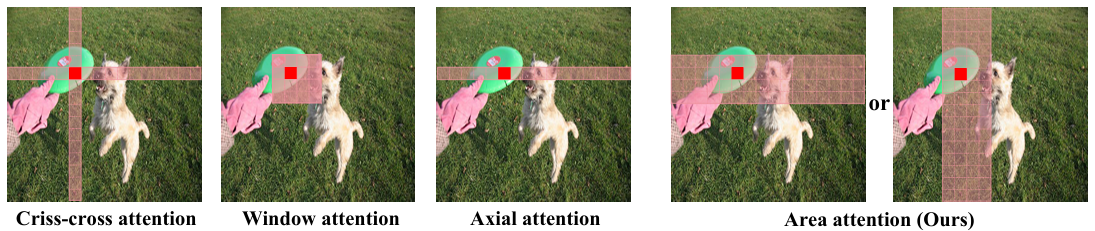
\includegraphics[width=0.9\textwidth]{images/YOLO1.png}
        \caption{Area attention mechanism in YOLOv12 compared to traditional attention mechanisms.}
        \label{fig:YOLOv12_attention}
    \end{figure}
    \item \textbf{R-ELAN}: A modified version of the ELAN architecture that improves optimization stability and convergence in deeper attention-based models, enabling YOLOv12 to scale effectively (Figure \ref{fig:YOLOv12_R-ELAN}).
    \begin{figure}[h]
        \centering
        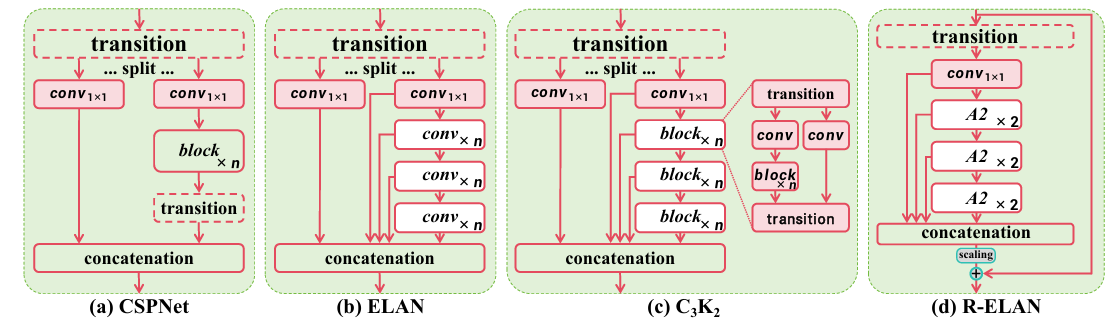
\includegraphics[width=0.9\textwidth]{images/YOLO2.png}
        \caption{YOLOv12 R-ELAN architecture overview, illustrating the skip connection mechanism to improve optimization stability in deeper attention-based models \cite{tian_yolov12_2025}.}
        \label{fig:YOLOv12_R-ELAN}
    \end{figure}
    \item \textbf{FlashAttention}: An efficient implementation of attention that reduces memory-access overhead during inference, further contributing to YOLOv12's low latency.
\end{itemize}

The main appeal of YOLOv12 in the context of this thesis is its excellent latency--accuracy trade-off and its ability to achieve strong results without depending on additional large-scale pretraining strategies. This makes it an attractive candidate whenever extremely low inference time is the primary design criterion. In addition, YOLOv12 is conceptually important because it shows that attention mechanisms can be integrated effectively even within the traditionally convolution-centric YOLO family, thereby challenging the assumption that attention is necessarily too slow for real-time detection \cite{tian_yolov12_2025}.

At the same time, YOLOv12 presents some practical limitations for the specific selection process carried out in this thesis. Its efficiency gains partly depend on hardware support for FlashAttention, which is not equally available across all deployment environments. Furthermore, according to the comparative evidence discussed in the DEIMv2 paper, DEIMv2 later surpassed YOLOv12 in the performance--cost trade-off, achieving higher detection accuracy with fewer parameters and lower computational cost in corresponding regimes \cite{huang_real-time_2026,tian_yolov12_2025}, as showed in Figure \ref{fig:DEIMvsYOLO}. For this reason, YOLOv12 was regarded as a strong benchmark and a valuable reference point, but not as the final choice for deployment.
\begin{figure}[h]
    \centering
    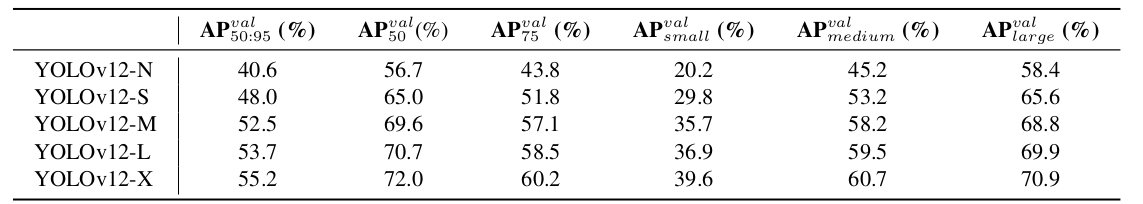
\includegraphics[width=0.9\textwidth]{images/YOLO_results.png}
    \caption{Summary of YOLOv12 results on the COCO benchmark, highlighting its strong balance between detection accuracy and inference efficiency across model scales \cite{tian_yolov12_2025}.}
    \label{fig:YOLOv12_Results}
\end{figure}
